\documentclass[twocolumn,english,notitlepage]{article}
\usepackage[margin=0.5in]{geometry}
\setlength{\parindent}{0pt} % no indents

% Math
\usepackage{amsmath}
\usepackage{physics}
\usepackage{amsfonts} % for mathbb

% Citetations
\usepackage[ backend=bibtex, sorting=none, autocite=plain]{biblatex}
\addbibresource{refs/references}
\usepackage{xcolor}
\usepackage{hyperref}
\hypersetup{
    colorlinks,
    linkcolor={red!50!black},
    citecolor={blue!50!black},
    urlcolor={blue!80!black}}


% Formatting
\usepackage{float}
\usepackage{graphicx}
\graphicspath{ {./figs/} } 

% Misc
\usepackage{appendix}

% Commands

\newcommand{\integral}[1]{\ensuremath{\int\!\mathrm{d}#1\,}}
\renewcommand{\d}[2][x]{\ensuremath{\frac{\mathrm{d}#2}{\mathrm{d}#1}}}

\renewcommand{\vec}[1]{\boldsymbol{#1}}
\newcommand{\pclosed}[1]{\left(#1\right)}
\newcommand{\bclosed}[1]{\left[#1\right]}
\newcommand{\cclosed}[1]{\left\{#1\right\}}
\newcommand{\vclosed}[1]{\left|#1\right|}
\renewcommand{\exp}[1]{e^{#1}}

\renewcommand{\expval}{\operatorname{\mathbb{E}}}
\renewcommand{\var}{\operatorname{Var}}
\DeclareMathOperator{\eye}{\mathbb{I}}

\newcommand{\betahat}{\hat{\beta}}

\title{An introduction to linear regression and variations} % very much working title
\author{Anna Aasen, Carl Martin Fevang, Håkon Kvernmoen}
\date{\today}

\begin{document}
\maketitle

\section{Introduction}

\begin{figure}[H]\label{fig:intro:plat}
    \centering
    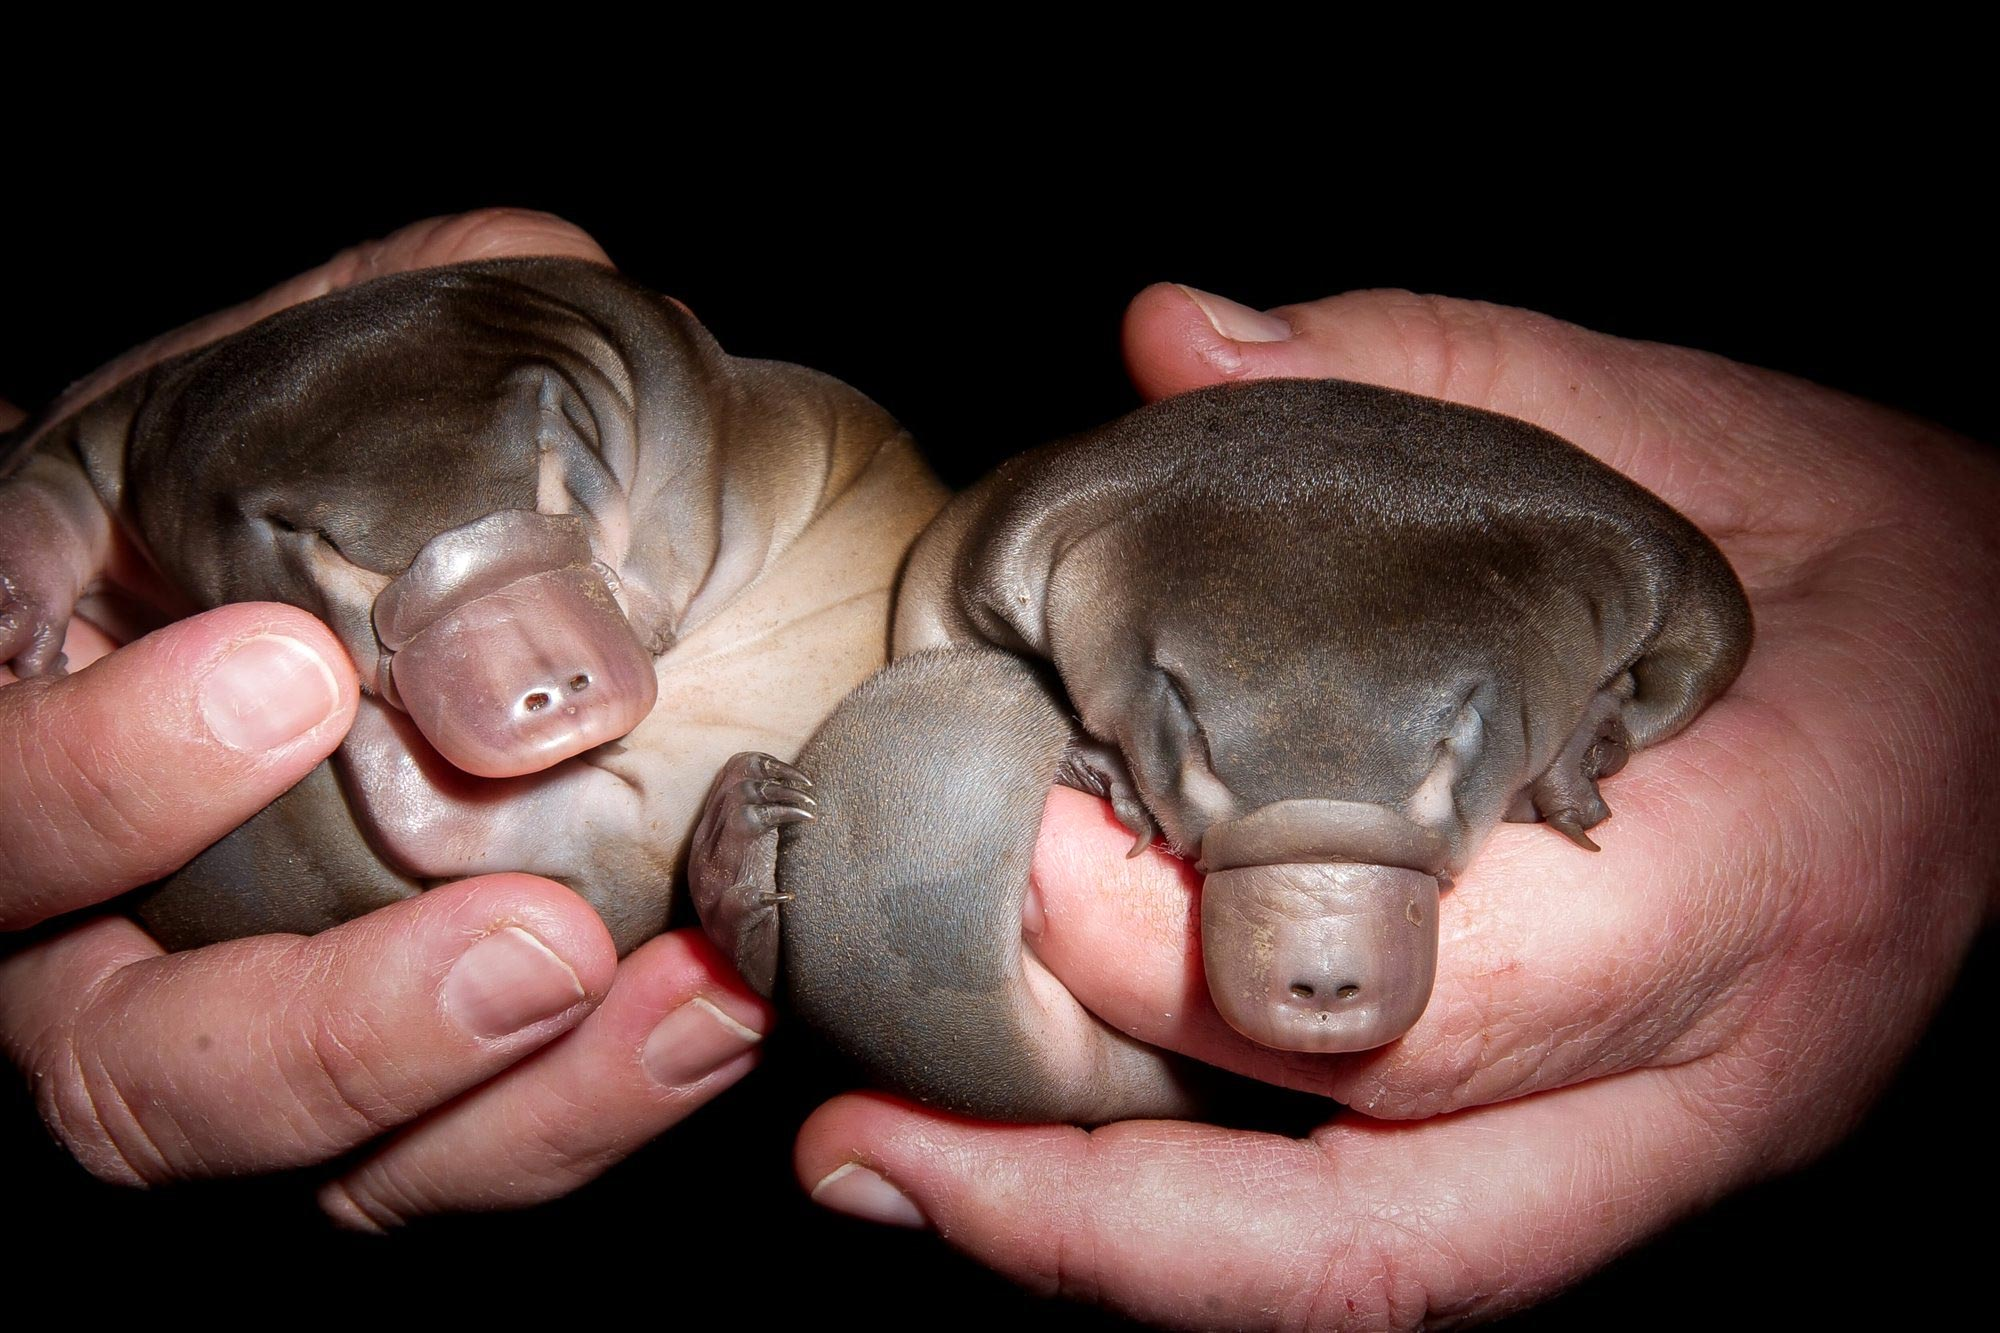
\includegraphics[width=0.5\linewidth]{Young-Platypus.jpg}
    \caption{Some figure caption}
\end{figure}

\section{Theory}
    \subsection{Statistical introduction to linear regression}
        A way to motivate the process of statistical learning is that we want to develop a process by which we use observed data to inform our belief in a future outcome. Such a process can be developed from the ideas of Bayes' theorem, which we can use to inform us what confidence we should have in the parameters of a given model, given data points we have observed.
        
        Let $\vec{y}$ denote a vector of a series of measured values $y_i$ at points $X$, where $X$ is a matrix where the rows $x_i$ correspond to the input values for the measurement $y_i$. Further let $\vec{\theta}$ denote the parameters of our given model -- then Bayes' theorem tells us that our \textit{posteriori} confidence in the parameters $\vec{\theta}$ given the available data follows
        \begin{align}
            P(\vec{\theta}|X, \vec{y}) = \frac{P(\vec{y}|X,\vec{\vec{\theta}})P(\vec{\theta})}{P(X,\vec{y})}.
        \end{align}
        Here $P(X,\vec{y})$ plays the role of a normalisation, and can safely be ignored -- either because we look for values of $\vec{\theta}$ that maximise the probability, or because we assume the probabilities $P(\vec{y}|X,\vec{\theta})$ and $P(\vec{\theta})$ which we then can properly normalise. Now we have a framework through which we can use assumptions about the distributions $P(\vec{y}|X,\vec{\theta})$ and $P(\vec{\theta})$ to give us a probability distribution for the parameters $\vec{\theta}$ that we can maximise.

        \subsubsection{Ordinary least squares}
            Now we can define the ordinary least squares method by assuming that the data $y$ that we want to make a fit to has a linear noise term that is normally distributed with mean nought. That is $y(x) = f(x) + \epsilon$, where $f(x)$ is some analytic, non-stochastic function of the data input $x$, and $\epsilon \sim N(0, \sigma^2)$. This means that if we make a model fitting $y(x)$ by a $\tilde{y}(x)$, we should expect the error at every data point $(y_i, x_i)$ to be be normally distributed with the same variance. In mathematical terms, we should expect
            \begin{align}
                P(\vec{y}|X, \vec{\theta}) = \prod_{i=0}^{n-1} \frac{1}{\sqrt{2\pi\sigma^2}} \exp{-\frac{{(y_i-\tilde{y}_i)}^2}{2\sigma^2}}.
            \end{align}
            Furthermore, we assume the parameters $\vec{\theta}$ to be distributed evenly, and as such, $P(\vec{\theta})$ just contributed to an overall normalisation. This means that maximising $P(\vec{y}|X, \vec{\beta})$ amounts to the same as maximising $P(\vec{\theta}|X, \vec{y})$, and can be done analytically.

            Knowing that the Gaussian distribution has a single extremum that is a maximum, we can find the values for $\vec{\theta}$ maximising the probability as
            \begin{align} \nonumber
                \d[\theta_k]{P(\vec{y}|X,\vec{\theta})} &= 0 \\
                \Rightarrow \prod_{i=0}^{n-1} \frac{1}{\sqrt{2\pi\sigma^2}} \frac{1}{\sigma^2} X_{ki}(y_i-X_{ij}\theta_j) \exp{-\frac{{(y_i - X_{ij}\theta_j)}^2}{2\sigma^2}} &= 0,
            \end{align}
            which as we can see, is maximisable point by point. This means that the optimal parameters $\vec{\hat{\theta}}_\text{OLS}$ that maximise $P(\vec{y}|X, \vec{\theta})$ can be found as
            \begin{align}
                \vec{\hat{\theta}}_\text{OLS} = \pclosed{X^TX}^{-1} X^T \vec{y}
            \end{align}.


        \subsection{Ridge regression and Lasso}
            So far, we have assumed that the parameters $\vec{\theta}$ are uniformly distributed, and as such have no \textit{bias} towards any particular value. In practice, this means that the OLS model will contort to fit itself to all values in the data. As such, a motivation for adding a bias could be for the sake of stability in the fit. This is done in ridge regression, where one assumes that the parameters are normally distributed, such that parameter values far from the mean are thought less likely to occurr. This in practice means that the model is less willing to contort to outliers in the dataset, trading it for a bias towards certain parameter values. Assuming the probability distrbution for $\vec{\theta}$
            \begin{align}
                P(\vec{\theta}) = \prod_{i=0}^{n-1} \frac{1}{\sqrt{2\pi\tau^2}} \exp{-\frac{\vec{\theta}^2}{2\tau^2}}
            \end{align}

            \begin{align}
                \vec{\hat{\theta}}_\text{ridge} = \pclosed{X^TX + 2\lambda \sigma^2}^{-1} X^T\vec{y}
            \end{align}



    \begin{align}
        \expval(y_i) = \expval\bclosed{X_{ij} \vec{\beta}_j + \epsilon_i} = X_{ij}\vec{\beta}_j + \expval(\epsilon) = X_{ij}\vec{\beta}_j
    \end{align}

    \begin{align} \nonumber
        \var(y_i) &= \expval\bclosed{\pclosed{y_i-\expval\pclosed{y_i}}^2} = \expval\bclosed{\pclosed{X_{ij}\vec{\beta}_j + \epsilon_i - X_{ij}\vec{\beta}_j}^2} \\
        &= \expval\pclosed{\epsilon_i^2} = \var\pclosed{\epsilon_i} = \sigma^2
    \end{align}

    \begin{align} \nonumber
        \expval(\vec{\betahat}) &= \expval\pclosed{(X^TX)^{-1}X^T \vec{y}} = \expval\pclosed{(X^TX)^{-1}X^T \bclosed{X\vec{\beta} + \vec{\epsilon}} } \\
        &= \expval\pclosed{\vec{\beta}} + {(X^TX)}^{-1}X^T \expval\pclosed{\vec{\epsilon}} = \vec{\beta}
    \end{align}

    \begin{align} \nonumber
        \var(\vec{\betahat}) &= \expval({\vec{\betahat} \vec{\betahat}^T}) - \expval({\vec{\betahat}}) \expval({\vec{\betahat}^T}) \\ \nonumber
        &= \expval((X^TX)^{-1}X^T \vec{y} \vec{y}^T X (X^TX)^{-1}) - \vec{\beta}\vec{\beta^T} \\ \nonumber
        &= (X^TX)^{-1}X^T \bclosed{X\vec{\beta}\vec{\beta}^TX^T + \sigma^2 \eye}X (X^TX)^{-1} - \vec{\beta}\vec{\beta}^T \\
        &= \sigma^2 (X^TX)^{-1},
    \end{align}
    where we have used that \(\expval(\vec{y}\vec{y}^T) = \expval\pclosed{(X\vec{\beta}+\vec{\epsilon})(X\vec{\beta}+\vec{\epsilon})^T} = X\vec{\beta}\vec{\beta}^TX^T + \sigma^2 \eye\).


\begin{appendix}
    \section{Appendix entry}
    some appendix things
\end{appendix}

\printbibliography

\end{document}

